%%%%%%%%%%%%%%%%%%%%%%%%%%%%%%%%%%%%%%%%%
%% Appendix section
% Set-up the section.
\newpage
\appendix
\setcounter{table}{0}
\renewcommand{\thetable}{A\arabic{table}}
\setcounter{figure}{0}
\renewcommand{\thefigure}{A\arabic{figure}}

% Start appendix
\section{Appendix}
\label{appendix}
This project used data which are fully public, and computational tools which are fully open-source.
As such, all code and data (anonymised versions where necessary) involved in this project are available at this project's Github repository, available at \url{https://github.com/shoganhennessy/state-faculty-composition}.
They may be used for replication, or as the basis for further work, as needed.
Any comments or suggestions may be sent to me at \href{mailto:seh325@cornell.edu}{\nolinkurl{seh325@cornell.edu}}, or raised as an issue on the Github project.

A number of statistical packages, for the $R$ language \citep{R2022}, made the empirical analysis for this paper possible.
\begin{itemize}
    \item \textit{Tidyverse} \citep{tidyverse} collected tools for data analysis in the $R$ language.
    \item \textit{LFE} \citep{lfe} implemented linear fixed effect models, with instruments, crucial for the empirical estimation in \autoref{sec:empirics}.
    \item \textit{Stargazer} \citep{stargazer} provided methods to efficiently convert empirical results into presentable output in \LaTeX.
    \item \textit{Lpirfs} \citep{lpirfs2019} implemented estimation of the \cite{jorda2005} local projections methods, with instrumental variables, crucial to the local projections estimates presented in this project.
\end{itemize}

\subsection{IPEDS First Stage}
\label{sec:appendix-ipeds-firststage}

\begin{table}[H]
    \singlespacing
    %\centering
    \caption{Shift-Share Instrument Balance, Mean Characteristics Across Instrument Distribution.}
    \makebox[\textwidth][c]{% latex table generated in R 4.3.3 by xtable 1.8-4 package
% Tue Sep 17 11:44:31 2024
\begin{tabular}{lccccc}
  \hline
Instrument Quantile: & 1st & 2nd & 3rd & 4th & 5th \\ 
  \hline
IV Components, \$ per student: &  &  &  &  &  \\ 
  Funding shift--share & -1,473.7 & -2,589.5 & -3,566.4 & -5,002.1 & -8,208.1 \\ 
  Shift in state--wide funding & -6,138.0 & -7,111.6 & -8,593.2 & -10,575.5 & -14,017.6 \\ 
  Share reliance on state funding, \% in 1990--1993 & 25.7 & 37.8 & 42.4 & 47.9 & 59.0 \\ 
  \hline University Funding and Spending, \$ millions: &  &  &  &  &  \\ 
  State funding & 110.3 & 99.2 & 99.8 & 107.1 & 107.1 \\ 
  Tuition revenue & 216.5 & 124.2 & 93.2 & 77.0 & 58.0 \\ 
  Total non-inst. revenues & 355.4 & 241.0 & 203.4 & 190.8 & 169.6 \\ 
  Instruction spending & 219.0 & 139.4 & 108.1 & 100.8 & 92.9 \\ 
  Research Spending & 150.0 & 74.6 & 53.9 & 35.9 & 25.5 \\ 
  \hline University Funding and Spending, \$ per student &  &  &  &  &  \\ 
  State funding & 12,900.1 & 9,956.2 & 9,334.7 & 9,304.9 & 12,766.7 \\ 
  Tuition revenue & 13,129.7 & 8,530.4 & 6,874.6 & 6,046.5 & 5,507.4 \\ 
  Total non-inst. revenues & 30,501.7 & 20,393.8 & 17,194.5 & 15,876.6 & 18,822.8 \\ 
  Instruction spending & 21,680.2 & 12,526.0 & 9,798.1 & 8,482.0 & 9,953.2 \\ 
  Research spending & 16,750.0 & 5,092.8 & 3,327.7 & 2,226.0 & 2,432.4 \\ 
  \hline Selectivity: &  &  &  &  &  \\ 
  Reported enrolment & 14,087.6 & 12,433.8 & 11,328.8 & 11,546.2 & 10,252.9 \\ 
  Full-time equivalent enrolment & 12,452.8 & 10,597.3 & 9,638.4 & 9,876.6 & 8,554.9 \\ 
  Acceptance rate, \% & 70.7 & 73.2 & 70.8 & 64.5 & 60.2 \\ 
  6 Year graduation rate, \% & 55.6 & 47.3 & 44.1 & 44.7 & 45.2 \\ 
   \hline
\end{tabular}
}
    \label{tab:summary-quantiles}
    \justify
    \footnotesize
    \textbf{Note}:
    This table shows the summary statistics for every public university--year observation in IPEDS data, for each of the 5 quantiles of the funding shift-share instrument.
    Funding shift-share is the instrument defined in \autoref{sec:empirics} the product of (1) state-wide funding shift and (2) share reliance on state funding.
    State-wide funding shift is total funding for higher education in that university's state (divided by the count of state students); share reliance on state funding is the the total amount of state funding received by the university in 1990--1993 divided by total revenues for those years. 
    The column labelled ``1st'' refers to the mean for all university-year observations in the first quintile (bottom 20\%) of the funding shift-share distribution, and so on.
    The numbers are adjusted to 2021 figures by CPI-U.
    Non-institutional revenues refers to the sum of federal, state, and local funding plus tuition revenues; these sum to the majority of university funding, but exclude numbers such as university income from capital projects.
    Acceptance rate and 6 year graduation rate are for university undergraduates, and are calculated from IPEDS data available for academic years 1997 through 2018.
\end{table}

\begin{figure}[H]
    \centering
    \singlespacing
    \caption{Correlation Between State Funding Shift-Share and Public University State Funding in Surrounding Years.}
    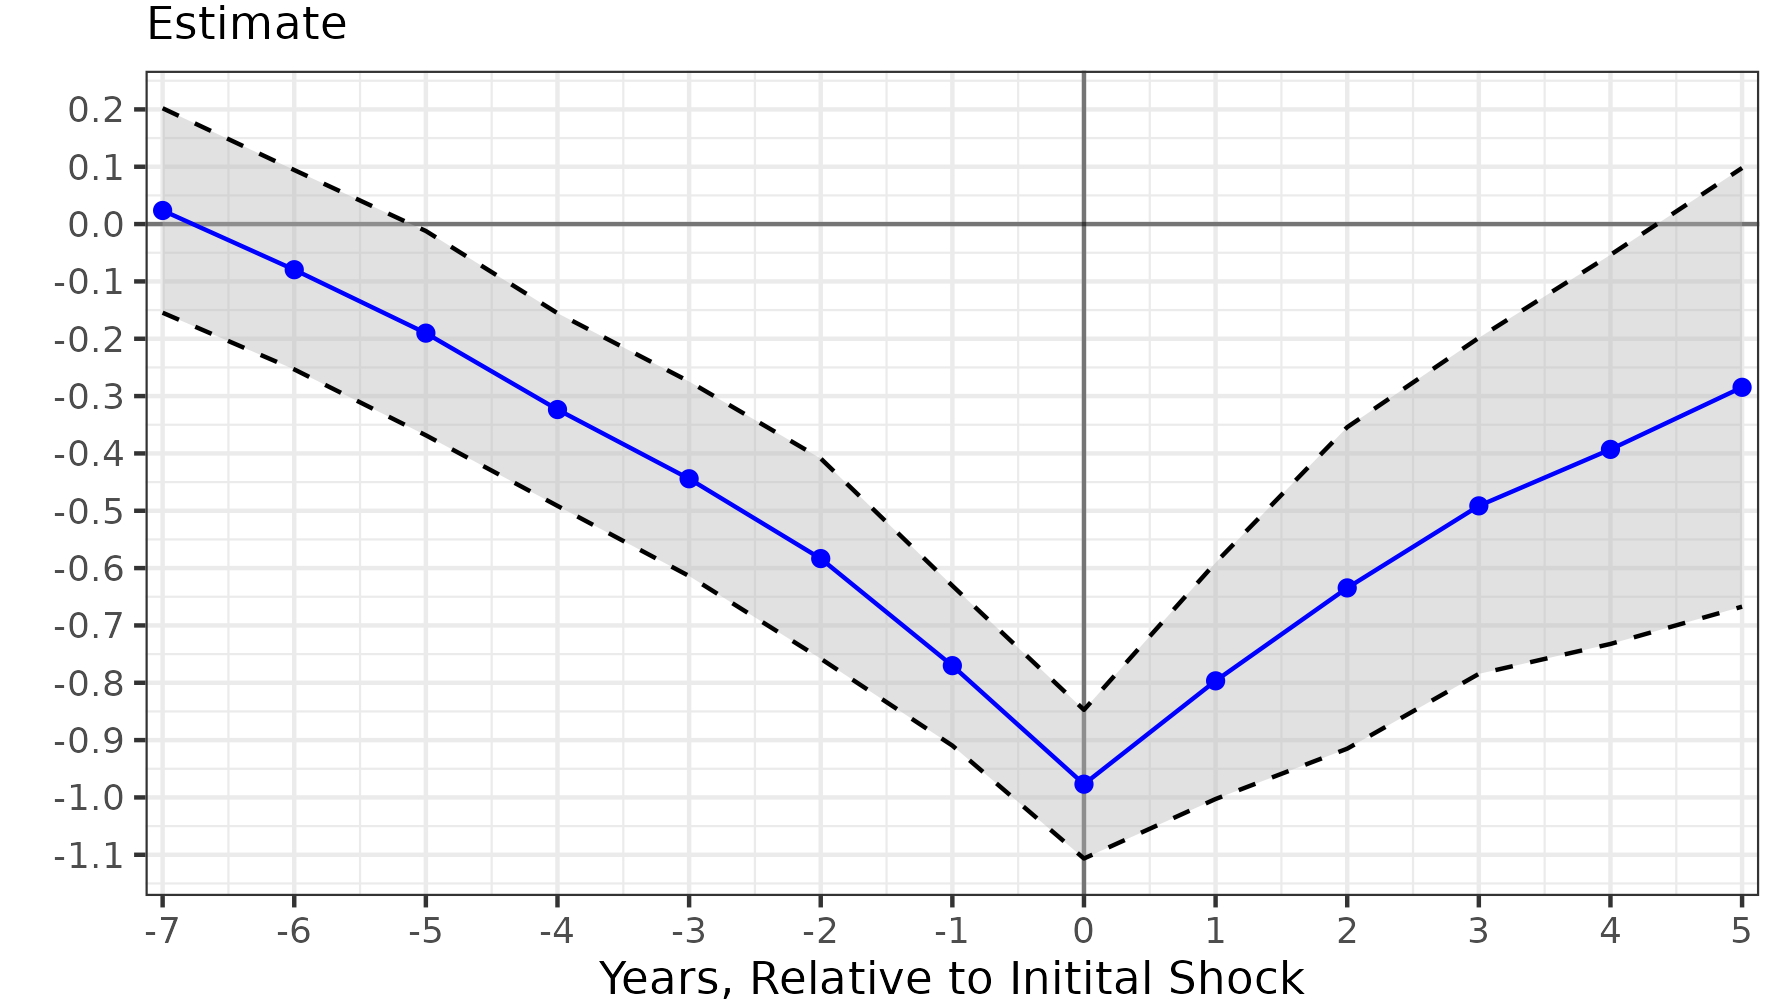
\includegraphics[width=\textwidth]{figures/lag-firststage.png}
    \label{fig:lag-firststage}
    \justify
    \footnotesize
    \textbf{Note}:
    This figure shows the correlation between state funding in year $t+k$ with the funding shift-share in year $t$ for a university, where $k = -7, \hdots, 5$ are the years on the $x$-axis.
    This shows that state funding and the funding shift-share are correlated across years, so that dynamic effects must be estimated by local projections --- and not simple OLS or 2SLS.
    The estimates are of \eqref{eqn:firststage}, calculated with IPEDS data, separately for each year relative to initial shock, using the $\log-\log$ specification, including fixed effects for university $+$ year, and clustering standard errors by university $+$ year.
\end{figure}

\begin{figure}[H]
    \centering
    \singlespacing
    \caption{Local Projection Estimates for Funding Shift-Share on State Funding, in IPEDS Data.}
    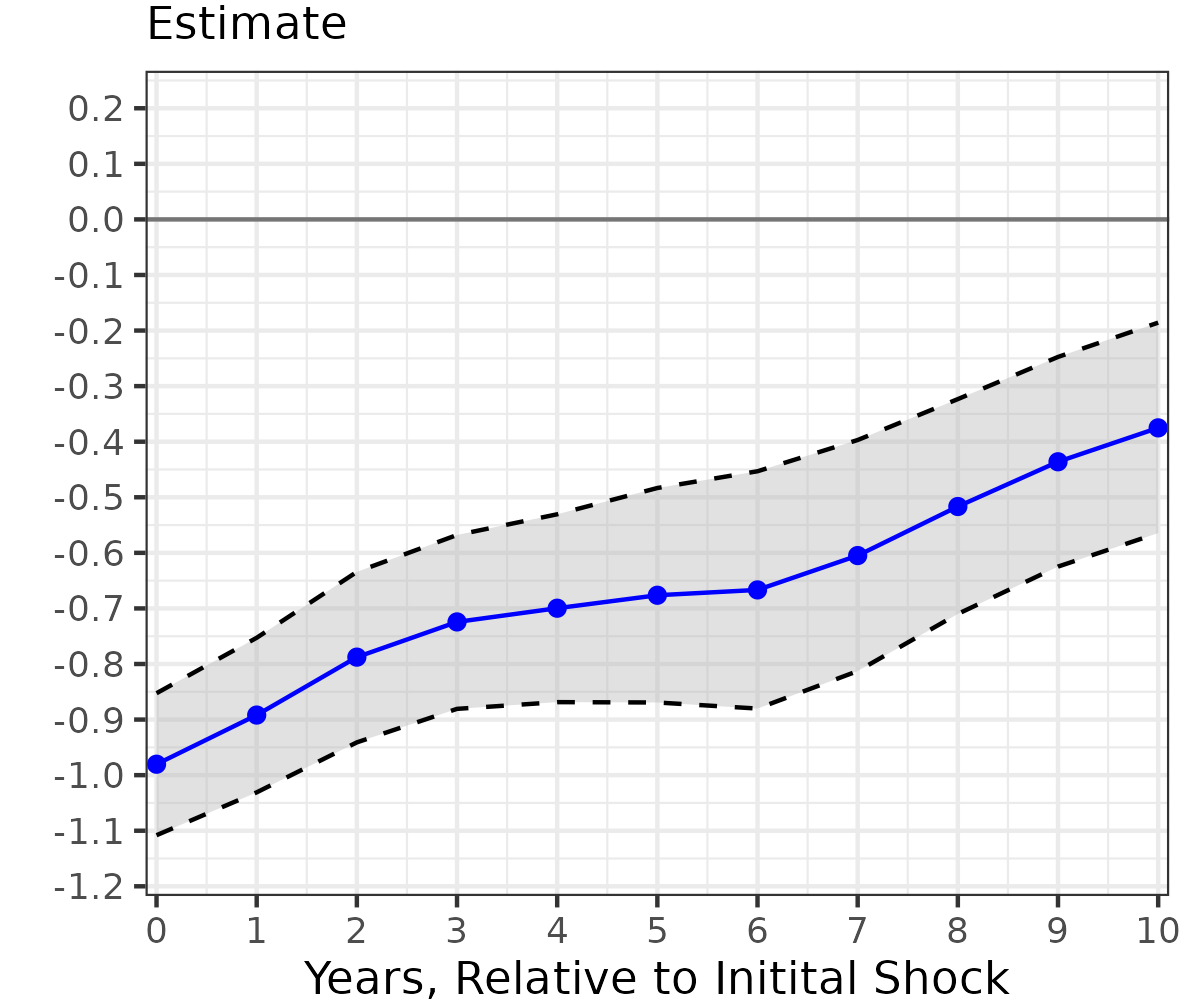
\includegraphics[width=0.6\textwidth]{figures/firststage-lp.png}
    \label{fig:firststage-lp}
    \justify
    \footnotesize
    \textbf{Note}:
    These figures show the local projections estimates of regression specification \eqref{eqn:firststage}, with the funding shift-share as an instrument for state funding, using IPEDS data.
    The coefficient estimate is effect of funding shift-share ($Z_{i,t}$) on state funding ($X_{i,t}$), while accounting for auto-correlation between different time periods --- i.e., between $Z_{i,t}, Z_{i,t-1}$ and $X_{i,t}, X_{i,t-1}$.
    These results use a $\log-\log$ specification, so the estimates are for the elasticity of state funding per student in a year $t+k$ with respect to funding shift-share in year $t$, where years $k = 0, \hdots, 10$ are on the $x$-axis. 
    Standard errors are clustered at the state-year level.
\end{figure}

\newpage
\subsection{Illinois IBHED First Stage}
\label{sec:iv-model-indiv}

This paper uses data on individual professors in the Illinois university system, to investigate the effects of changes in university revenues on the individual professors at the universities.
The outcomes here now refer to individual professors (e.g., their salary and promotion rate), so requires adjustment to the empirical approach, leveraging variation in university funding for the years after a professor joins the university.

\autoref{eqn:rolling-instrument} defines a rolling-share variant of the instrument, $\tilde Z_{i(j),t}$, where the university's state funding share exposure is based in the year a professor joins the university --- and not the base period 1990--1993.
$j$ indexes each professor in year $t$, $\tau(j)$ for the year the professor first joins their institution.
Identifying $\tau(j)$ is possible for $j$ by restricting to all professors hired 2011-2021 --- i.e., in the years after the start of the full panel.
It is not possible to discern the hiring year for professors who  were hired in the years preceding 2011, and so the entire sample is only possible to analyse using the base-share in years 1990-1993 formulation.

\begin{align}
    \label{eqn:rolling-instrument}
    \tilde Z_{i(j),t} &\coloneqq - \left[
    \left( \frac{\text{Total State Funding}_{s(j),t}}{\text{Student Population}_{s(j),t}} \right)
    \left( \frac{\text{State Funding}_{\tau(j)}}{\text{Total Revenues}_{i,\tau(j)}} \right) \right]
\end{align}

This approach leverages an insight, made available by level of the data: that an individual professor is affected by changes in university revenues after they have joined the university.
\autoref{sec:iv-model-uni} considers the number of professors employed by the university; whether a professor becomes employed at the university is likely affected by that university's finances.
The formulation here takes as given that the professor is already employed at the university, and then projects the effect of changes in state funding on these \textit{incumbent} professors following the state funding shift-share.
\autoref{tab:firststage-illinois} presents the first-stage results in Illinois data.

\begin{table}[h!]
    \singlespacing
    \centering
    \caption{First Stage Estimates, for State Funding by Funding Shift-Share in IBHED Data.}
    \textbf{Panel A: units in \$ per student}
    
    \makebox[\textwidth][c]{
\begin{tabular}{@{\extracolsep{5pt}}lcccc} 
\\[-1.8ex]\hline 
\hline \\[-1.8ex] 
 & \multicolumn{4}{c}{Dependent Variable: State Funding} \\ 
\cline{2-5} 
\\[-1.8ex] & (1) & (2) & (3) & (4)\\ 
\hline \\[-1.8ex] 
 Funding Shock & $-$1.176 & $-$0.160 & $-$1.100 & $-$1.071 \\ 
  & (0.226) & (0.265) & (0.242) & (0.264) \\ 
  Tuition Revenue &  &  & $-$0.295 & 1.012 \\ 
  &  &  & (0.136) & (0.329) \\ 
  Constant &  & 9,716.437 &  & $-$1,708.334 \\ 
  &  & (1,805.394) &  & (2,716.150) \\ 
 \hline \\[-1.8ex] 
Uni. + Year fixed effects? & Yes & No & Yes & No \\ 
F stat. & 20.712 & 16.512 & 26.999 & 0.365 \\ 
Observations & 17,012 & 17,012 & 17,012 & 17,012 \\ 
R$^{2}$ & 0.918 & 0.0004 & 0.919 & 0.074 \\ 
\hline 
\hline \\[-1.8ex] 
\end{tabular} 
}
    
    \textbf{Panel A: units in log \$ per student}
    
    \makebox[\textwidth][c]{
\begin{tabular}{@{\extracolsep{5pt}}lcccc} 
\\[-1.8ex]\hline 
\hline \\[-1.8ex] 
 & \multicolumn{4}{c}{Dependent Variable: State Funding} \\ 
\cline{2-5} 
\\[-1.8ex] & (1) & (2) & (3) & (4)\\ 
\hline \\[-1.8ex] 
  State Funding & $-$1.000 & $-$0.877 & $-$0.987 & $-$0.726 \\ 
  & (0.018) & (0.046) & (0.026) & (0.155) \\ 
  Tuition Revenue & 0.538 & 0.536 &  &  \\ 
  & (0.334) & (0.270) &  &  \\ 
  Constant &  & $-$3.298 &  & 3.004 \\ 
  &  & (2.477) &  & (1.259) \\ 
 \hline \\[-1.8ex] 
Fixed effects? & Yes & No & Yes & No \\ 
F stat. & 3118.566 & 364.133 & 1394.217 & 21.88 \\ 
Observations & 70,743 & 187,634 & 70,743 & 187,634 \\ 
R$^{2}$ & 0.928 & 0.521 & 0.924 & 0.414 \\ 
\hline 
\hline \\[-1.8ex] 
\end{tabular} 
}
    
    \label{tab:firststage-illinois}
    \justify
    \footnotesize
    \textbf{Note}:
    These tables show the first stage OLS estimates of regression specification \eqref{eqn:secondstage1_indiv}, showing the effect of the funding shift-share on state funding to gauge performance as an instrument.
    Each observation is a professor-year, in the IBHED data, and funding data are merged from IPEDS.
    %Panel A shows the effect of an funding shift-share of \$-1 per student in the state on the number of \$'s of state funding per student at the university --- i.e.,
    %\$-1 funding shift-share per student in the state leads to \$1.176 less state funding per student at the university according to preferred specification column 1.
    Panel A shows the effect of a $-10$\% change funding shift-share per student in the state on $10$\% change in state funding per student at the university --- i.e.,
    $-10$\% funding shift-share per student in the state leads to $-9.77$\% less state funding per student at the university according to prefferred specification column 1.        
    Standard errors are clustered at the institution-year level, and institution $+$ year fixed effects are included where noted.
\end{table}

Exogeneity and relevance of the rolling-share instrument, $\tilde Z_{i(j),t}$, follows the same reasoning as that for the base-share instrument, $Z_{i,t}$, discussed in \autoref{sec:approp-shocks}.
The base-share instrument is appropriate for some outcomes with the individual Illinois professors, where appropriate.
We satisfy the assumptions for exogeneity by noting that none of the Illinois public campuses take the majority of state funding, and that the identification strategy relies on exogeneity in changes in state funding to individual professor-outcomes, following the year they joined the university.
Additionally, within-institution changes resulting from share reliance on state funding may be correlated with unobserved changes in the outcomes, so that \cite{NBERw27885} note the importance of controlling for the base share and state student population.
The formulation here implicitly controls for these factors via the fixed effects; results are relatively similar while including these controls with and without including fixed effects, and so are omitted.

The instrumental variables model is then defined as follows, where $i(j)$ refers to the institution that professor $j$ is employed at, and $Y_{j,t}$ for salary, rate of promotion, and propensity to leave the Illinois public university system.
The system includes fixed effects for the institution and first year of employment.
The instrument varies by institution, based in the year of first employment, so that these are the corresponding fixed effects and level of clustered standard errors.
\begin{eqnarray}
    \label{eqn:secondstage1_indiv}
    X_{i(j),t} &=& \theta_{i(j)} + \phi_{\tau(j)} + \delta \tilde Z_{i(j),t} + \epsilon_{i(j),t} \\
    \label{eqn:secondstage2_indiv}
    Y_{j,t} &=& \mu_{i(j)} + \nu_{\tau(j)} + \beta \widehat X_{i(j),t} + \varepsilon_{j,t}
\end{eqnarray}
We then interpret parameter $\beta$ as the effect of changes in state funding at an Illinois public university, via state funding shift-shares, on an individual professor's outcome $Y_{j,t}$.

\newpage
\begin{figure}[H]
    \centering
    \singlespacing
    \caption{Local Projection Estimates for Effect of State Funding on Faculty Promotion Rate at Illinois Public Universities, by Professor Group.}
    \begin{subfigure}[b]{0.495\textwidth}
        \centering
        \caption{Lecturers.}
        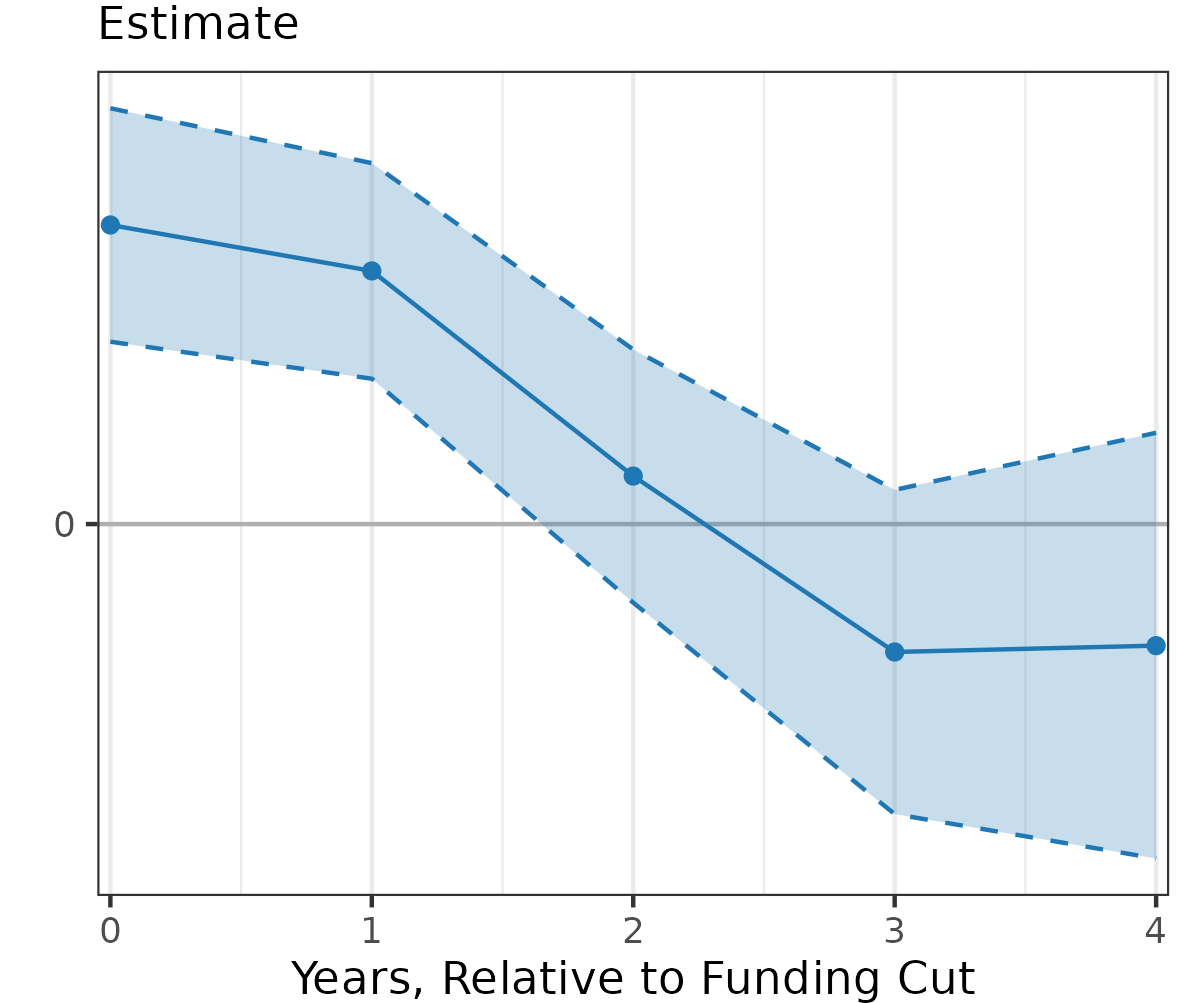
\includegraphics[width=\textwidth]{figures/promoted-lecturer-illinois-lp-rolling.png}
        \label{fig:promoted-lecturer-illinois-lp-rolling}
    \end{subfigure}
    \begin{subfigure}[b]{0.495\textwidth}
        \centering
        \caption{Assistant Professors.}
        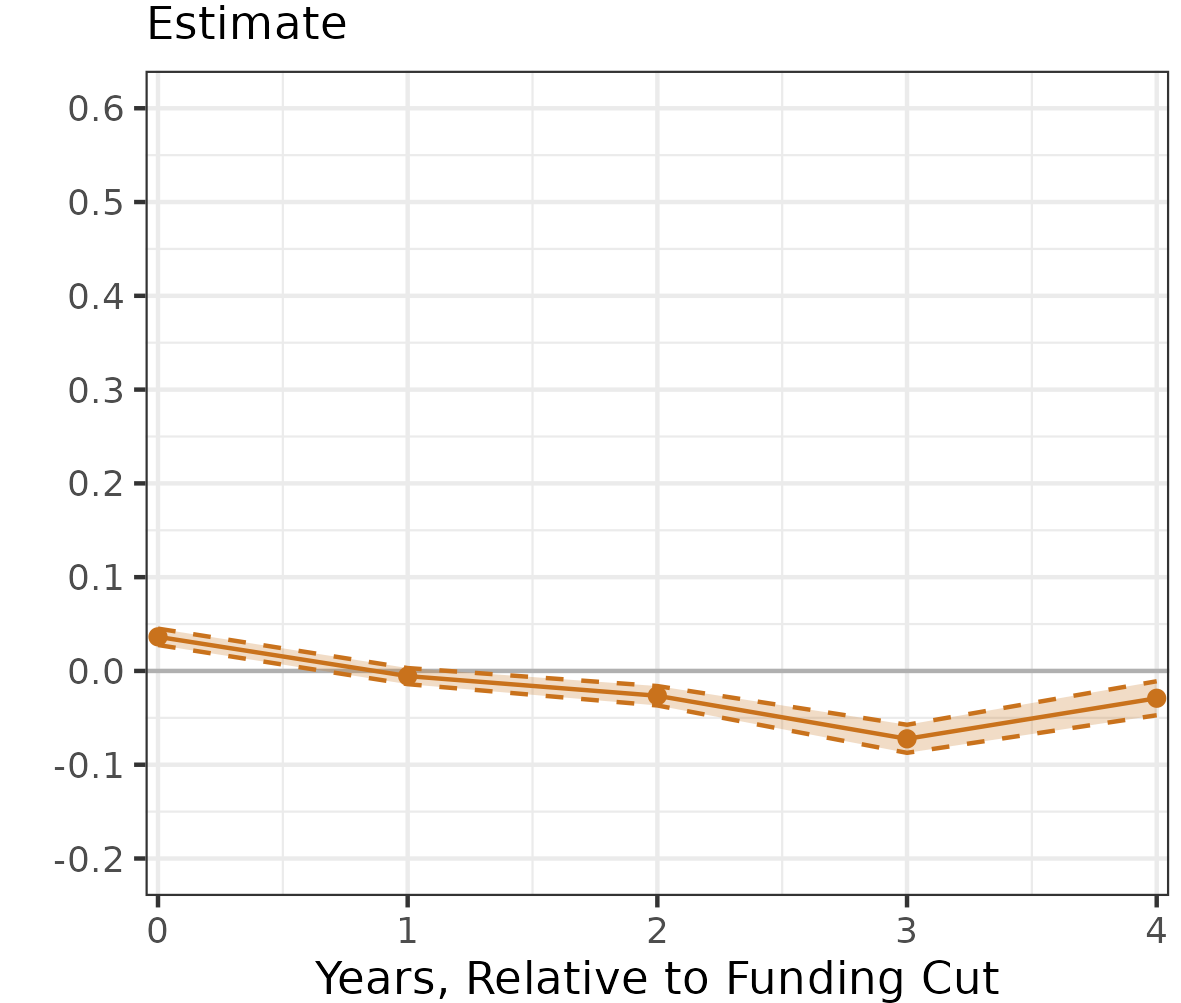
\includegraphics[width=\textwidth]{figures/promoted-assistant-illinois-lp-rolling.png}
        \label{fig:promoted-assistant-illinois-lp-rolling}
    \end{subfigure}
    \begin{subfigure}[b]{0.495\textwidth}
        \centering
        \caption{Full Professors.}
        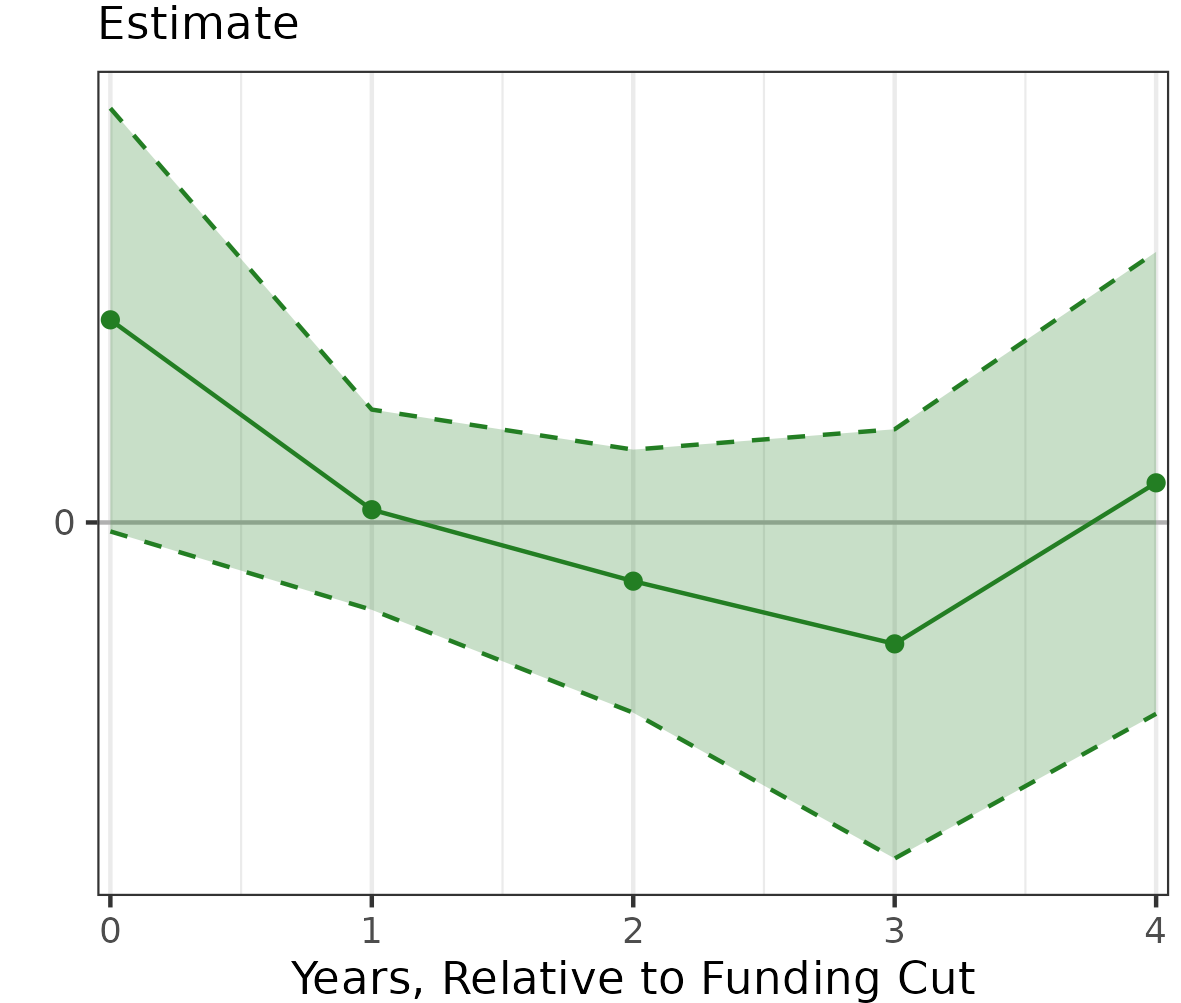
\includegraphics[width=\textwidth]{figures/promoted-full-illinois-lp-rolling.png}
        \label{fig:promoted-full-illinois-lp-rolling}
    \end{subfigure}
    \label{fig:promoted-illinois-lp-rolling}
    \justify
    \footnotesize
    \textbf{Note}:
    These figures show the local projections estimates of regression specification \eqref{eqn:secondstage}, with the funding shift-share as an instrument for state funding.
    The unit of analysis is an individual faculty member (at an Illinois public university); funding data come from IPEDS, and faculty promotion rate from IBHED.
    The coefficient estimate is effect of state funding ($X_{i(j),t}$) on faculty promotion rate ($Y_{j,t}$), using the funding shift-share instrument ($Z_{i(j),t}$), while accounting for auto-correlation between different time periods --- i.e., between $X_{i(j),t}, X_{i(j),t-1}$ and $Y_{i(j),t}, Y_{i(j),t-1}$.
    These results use a $\log-\log$ specification, so the estimates are for the rate of promotion in a year $t+k$ affected by a 1\% change in state funding in year $t$, where years $k = 0, \hdots, 4$ are on the $x$-axis. 
    Standard errors are clustered at the university-year level, and \autoref{sec:iv-model-indiv} fully describes the differences in empirical specification when unit of analysis is an individual faculty member.
\end{figure}

\newpage
\begin{table}[H]
    \singlespacing
    \centering
    \caption{Effects of Changes in State Funding on University Faculty Composition, in Illinois 2010--2021, OLS and 2SLS Estimates.}

    \textbf{Panel A: units in \$ per student}

    \makebox[\textwidth][c]{
\begin{tabular}{@{\extracolsep{5pt}}lcccccccc} 
\\[-1.8ex]\hline 
\hline \\[-1.8ex] 
 & \multicolumn{8}{c}{Dependent Variable: Employment Count by Professor Group} \\ 
\cline{2-9} 
\\[-1.8ex] & \multicolumn{2}{c}{Lecturer} & \multicolumn{2}{c}{Assistant} & \multicolumn{2}{c}{Full} & \multicolumn{2}{c}{All} \\ 
 & OLS & 2SLS & OLS & 2SLS & OLS & 2SLS & OLS & 2SLS \\ 
\\[-1.8ex] & (1) & (2) & (3) & (4) & (5) & (6) & (7) & (8)\\ 
\hline \\[-1.8ex] 
 State Funding & $-$3.729 & 0.376 & 0.415 & 3.208 & $-$1.269 & 0.117 & $-$4.084 & 3.890 \\ 
  & (1.721) & (1.725) & (1.728) & (2.493) & (1.548) & (1.200) & (4.352) & (5.668) \\ 
 \hline \\[-1.8ex] 
Outcome Mean & 351.306 & 351.306 & 273.757 & 273.757 & 477.597 & 477.597 & 1303.014 & 1303.014 \\ 
Observations & 144 & 144 & 144 & 144 & 144 & 144 & 144 & 144 \\ 
R$^{2}$ & 0.886 & 0.882 & 0.970 & 0.969 & 0.991 & 0.991 & 0.981 & 0.980 \\ 
\hline 
\hline \\[-1.8ex] 
\end{tabular} 
}
    
    \textbf{Panel B: units in log \$ per student}
    
    \makebox[\textwidth][c]{
\begin{tabular}{@{\extracolsep{5pt}}lcccccccc} 
\\[-1.8ex]\hline 
\hline \\[-1.8ex] 
 & \multicolumn{8}{c}{Dependent Variable: Employment Count by Professor Group} \\ 
\cline{2-9} 
\\[-1.8ex] & \multicolumn{2}{c}{Lecturer} & \multicolumn{2}{c}{Assistant} & \multicolumn{2}{c}{Full} & \multicolumn{2}{c}{All} \\ 
 & OLS & 2SLS & OLS & 2SLS & OLS & 2SLS & OLS & 2SLS \\ 
\\[-1.8ex] & (1) & (2) & (3) & (4) & (5) & (6) & (7) & (8)\\ 
\hline \\[-1.8ex] 
 State Funding & $-$0.015 & $-$0.017 & 0.049 & 0.058 & 0.007 & $-$0.029 & 0.004 & $-$0.008 \\ 
  & (0.033) & (0.026) & (0.045) & (0.038) & (0.021) & (0.032) & (0.028) & (0.022) \\ 
 \hline \\[-1.8ex] 
Outcome Mean & 2.523 & 2.523 & 1.491 & 1.491 & 2.729 & 2.729 & 8.141 & 8.141 \\ 
Observations & 144 & 144 & 144 & 144 & 144 & 144 & 144 & 144 \\ 
R$^{2}$ & 0.700 & 0.700 & 0.789 & 0.789 & 0.839 & 0.836 & 0.633 & 0.632 \\ 
\hline 
\hline \\[-1.8ex] 
\end{tabular} 
}

    \label{tab:facultycount-illinois-reg}
    \justify
    \footnotesize
    \textbf{Note}:
    These tables show the second stage OLS and 2SLS estimates of regression specification \eqref{eqn:secondstage}, showing the effect of state funding changes on number of faculty per student in Illinois universities, using the funding shift-share to instrument for state funding in the columns labelled 2SLS.
    Each observation is a public university-year in the state of Illinois, where funding data come from IPEDS and faculty count come from IBHED data.
    Panel A shows the effect of a fall in state funding \$$-1,000$ per student in the state on the number of professors.
    Panel B shows the effect of a $10$\% change in state funding per student at the university on the 10\% change in the number of professors per students.
    Outcome-mean is the mean of the outcome, for Panel A the number of professors per student, for Panel B the number of faculty per student.
    Panel B uses $\log$ faculty count per student as the outcome, though the outcome mean is count of faculty per student (not in $\log$ terms).
    Standard errors are clustered at the university-year level, and university $+$ year fixed effects are included through--out.
\end{table}

\newpage
\begin{figure}[H]
    \centering
    \singlespacing
    \caption{Local Projection Estimates for Effect of State Funding on Faculty Exit Rate at Illinois Public Universities, by Professor Group.}
    \begin{subfigure}[b]{0.495\textwidth}
        \centering
        \caption{Lecturers.}
        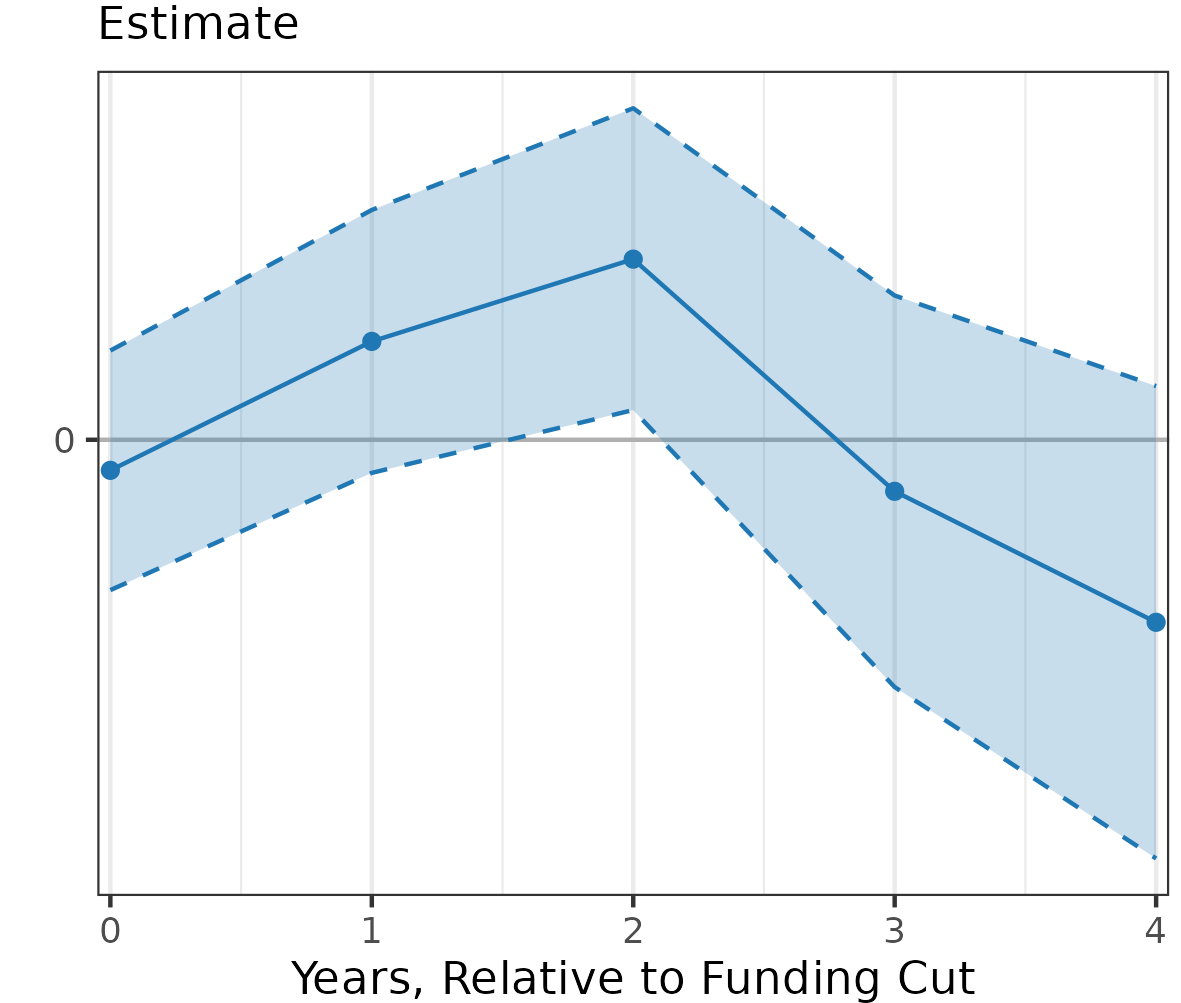
\includegraphics[width=\textwidth]{figures/exit-lecturer-illinois-lp-rolling.png}
        \label{fig:exit-lecturer-illinois-lp-rolling}
    \end{subfigure}
    \begin{subfigure}[b]{0.495\textwidth}
        \centering
        \caption{Assistant Professors.}
        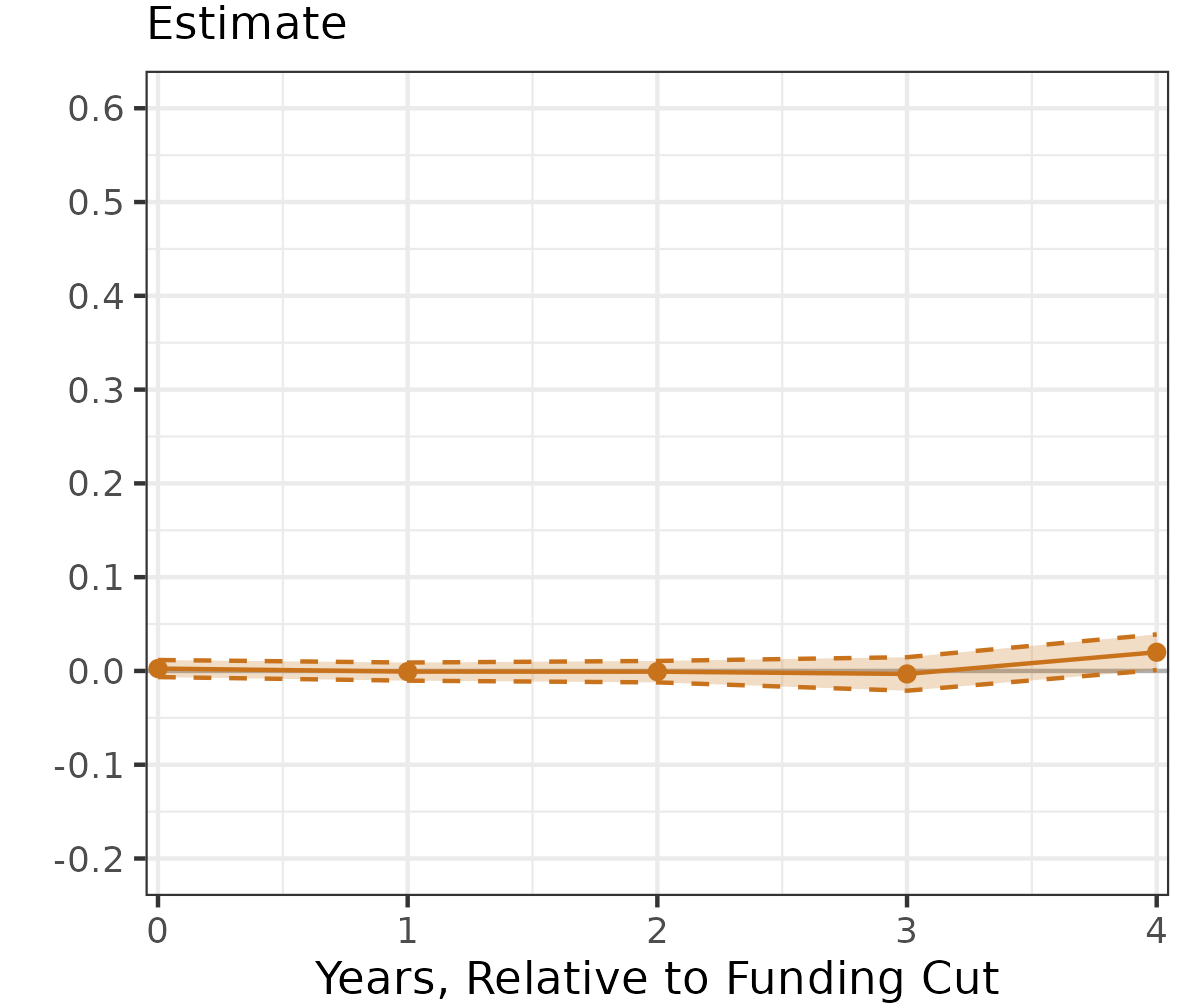
\includegraphics[width=\textwidth]{figures/exit-assistant-illinois-lp-rolling.png}
        \label{fig:exit-assistant-illinois-lp-rolling}
    \end{subfigure}
    \begin{subfigure}[b]{0.495\textwidth}
        \centering
        \caption{Full Professors.}
        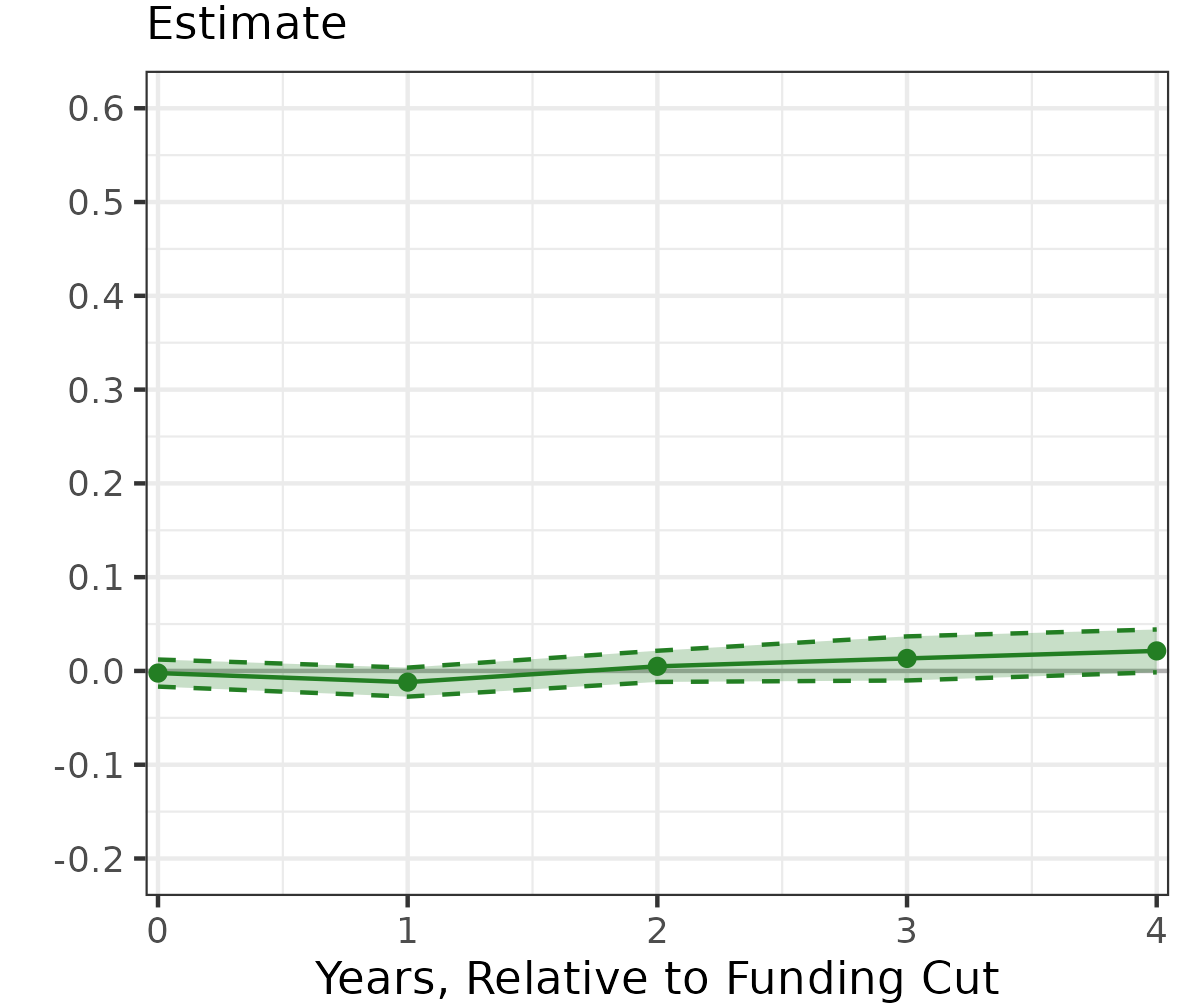
\includegraphics[width=\textwidth]{figures/exit-full-illinois-lp-rolling.png}
        \label{fig:exit-full-illinois-lp-rolling}
    \end{subfigure}
    \begin{subfigure}[b]{0.495\textwidth}
        \centering
        \caption{Administrator Professors.}
        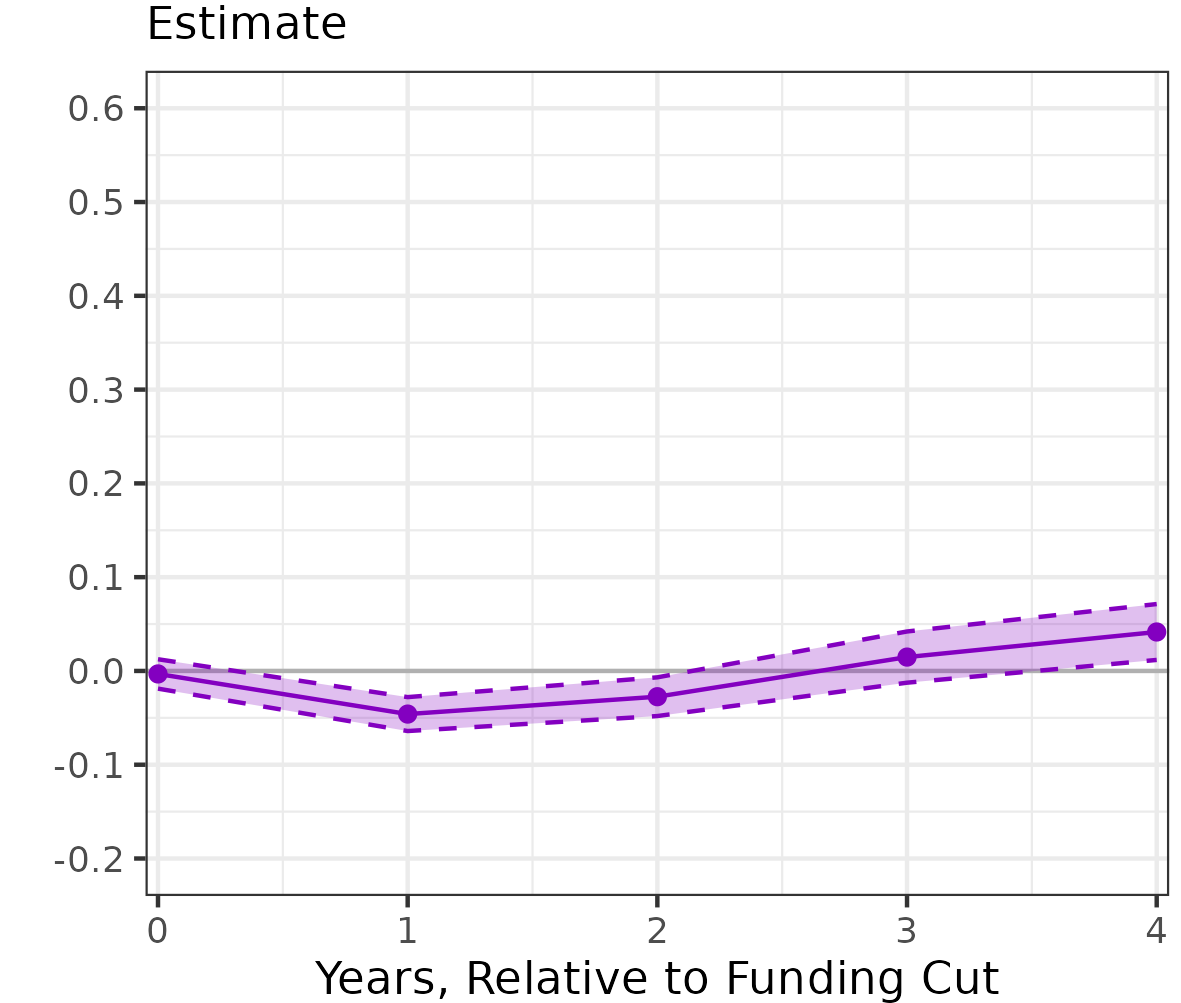
\includegraphics[width=\textwidth]{figures/exit-administrator-illinois-lp-rolling.png}
        \label{fig:exit-administrator-illinois-lp-rolling}
    \end{subfigure}
    \label{fig:exit-illinois-lp-rolling}
    \justify
    \footnotesize
    \textbf{Note}:
    These figures show the local projections estimates of regression specification \eqref{eqn:secondstage}, with the funding shift-share as an instrument for state funding.
    The unit of analysis is an individual faculty member (at an Illinois public university); funding data come from IPEDS, and faculty promotion rate from IBHED.
    The coefficient estimate is effect of state funding ($X_{i(j),t}$) on faculty promotion rate ($Y_{j,t}$), using the funding shift-share instrument ($Z_{i(j),t}$), while accounting for auto-correlation between different time periods --- i.e., between $X_{i(j),t}, X_{i(j),t-1}$ and $Y_{i(j),t}, Y_{i(j),t-1}$.
    These results use a rate$-\log$ specification, so the estimates are for the rate of promotion in a year $t+k$ affected by a 1\% change in state funding in year $t$, where years $k = 0, \hdots, 4$ are on the $x$-axis. 
    Standard errors are clustered at the university-year level, and \autoref{sec:iv-model-indiv} fully describes the differences in empirical specification when unit of analysis is an individual faculty member.
\end{figure}

\newpage
\subsection{Professor Hiring}
\label{sec:appendix-hiring}

These results were produced by integrating the total count of professor hires for 2010--2021 for the top-ranked 180 US universities with a sum of the funding variables, and then estimating the models specified in \autoref{sec:iv-model-uni}.
There were no observable differences in the hiring rate of male versus female faculty.

\begin{table}[H]
    \singlespacing
    \centering
    \caption{OLS and 2SLS Estimates for University Faculty Hires, in Illinois 2011--2021.}

    \textbf{Panel A: units in \$ per student}

    \makebox[\textwidth][c]{
\begin{tabular}{@{\extracolsep{5pt}}lcccccccc} 
\\[-1.8ex]\hline 
\hline \\[-1.8ex] 
 & \multicolumn{8}{c}{Dependent Variable: Yearly New Hires by Professor Group} \\ 
\cline{2-9} 
\\[-1.8ex] & \multicolumn{2}{c}{Lecturers} & \multicolumn{2}{c}{Asst. Professors} & \multicolumn{2}{c}{Full Professors} & \multicolumn{2}{c}{All Faculty} \\ 
 & OLS & 2SLS & OLS & 2SLS & OLS & 2SLS & OLS & 2SLS \\ 
\\[-1.8ex] & (1) & (2) & (3) & (4) & (5) & (6) & (7) & (8)\\ 
\hline \\[-1.8ex] 
 State Funding & $-$2.551 & $-$2.280 & 0.060 & $-$5.126 & $-$0.095 & $-$2.562 & $-$2.677 & 23.012 \\ 
  & (1.420) & (9.168) & (0.675) & (7.210) & (0.249) & (7.051) & (2.185) & (52.652) \\ 
 \hline \\[-1.8ex] 
Outcome Mean & 73.275 & 73.275 & 42.771 & 42.771 & 12.301 & 12.301 & 151.932 & 151.932 \\ 
Observations & 131 & 131 & 131 & 131 & 113 & 113 & 132 & 132 \\ 
R$^{2}$ & 0.839 & 0.839 & 0.934 & 0.902 & 0.788 & 0.752 & 0.918 & 0.793 \\ 
\hline 
\hline \\[-1.8ex] 
\end{tabular} 
}
    
    \textbf{Panel B: units in log \$ per student}
    
    \makebox[\textwidth][c]{
\begin{tabular}{@{\extracolsep{5pt}}lcccccccc} 
\\[-1.8ex]\hline 
\hline \\[-1.8ex] 
 & \multicolumn{8}{c}{Dependent Variable: Employment Count} \\ 
\cline{2-9} 
\\[-1.8ex] & \multicolumn{2}{c}{Lecturers} & \multicolumn{2}{c}{Asst. Professors} & \multicolumn{2}{c}{Full Professors} & \multicolumn{2}{c}{All Faculty} \\ 
 & OLS & 2SLS & OLS & 2SLS & OLS & 2SLS & OLS & 2SLS \\ 
\\[-1.8ex] & (1) & (2) & (3) & (4) & (5) & (6) & (7) & (8)\\ 
\hline \\[-1.8ex] 
 State Funding & 0.120 & 0.158 & 0.172 & 0.174 & 0.191 & 0.235 & 0.046 & 0.082 \\ 
  & (0.071) & (0.065) & (0.154) & (0.143) & (0.113) & (0.137) & (0.080) & (0.047) \\ 
 \hline \\[-1.8ex] 
Outcome Mean & 0.494 & 0.494 & 0.234 & 0.234 & 0.051 & 0.051 & 0.993 & 0.993 \\ 
Observations & 131 & 131 & 131 & 131 & 113 & 113 & 132 & 132 \\ 
R$^{2}$ & 0.749 & 0.749 & 0.482 & 0.482 & 0.628 & 0.627 & 0.580 & 0.579 \\ 
\hline 
\hline \\[-1.8ex] 
\end{tabular} 
}
    \label{tab:facultyhires-illinois-reg}
    \vspace{-0.5cm}
    \justify
    \footnotesize
    \textbf{Note}:
    These tables show the second stage OLS and 2SLS estimates of regression specification \eqref{eqn:secondstage}, showing the effect of state funding changes on number of faculty hires at Illinois universities, using the funding shift-share to instrument for state funding in the columns labelled 2SLS.
    Each observation is a public university-year in the state of Illinois, where funding data come from IPEDS and faculty count come from IBHED data.
    Panel A shows the effect of a fall in state funding \$$-1,000$ per student in the state on the number of new faculty hires by position.
    Panel B shows the effect of a $10$\% change in state funding per student at the university on the 10\% change in the number of faculty hires per students.
    Outcome-mean is the mean of the outcome, for Panel A the number of faculty hires, for Panel B the number of faculty hires per student.
    Panel B uses new faculty hires per student as the outcome (in $\log$ terms), though the outcome mean is count of new faculty hires per student (not in $\log$ terms).
    Standard errors are clustered at the university-year level, and university $+$ year fixed effects are included through--out.
\end{table}

\vspace{-0.5cm}
\begin{figure}[H]
    \centering
    \singlespacing
    \caption{Correlation Between State Funding and Total Count Professors Hired, 2011--2021.}
    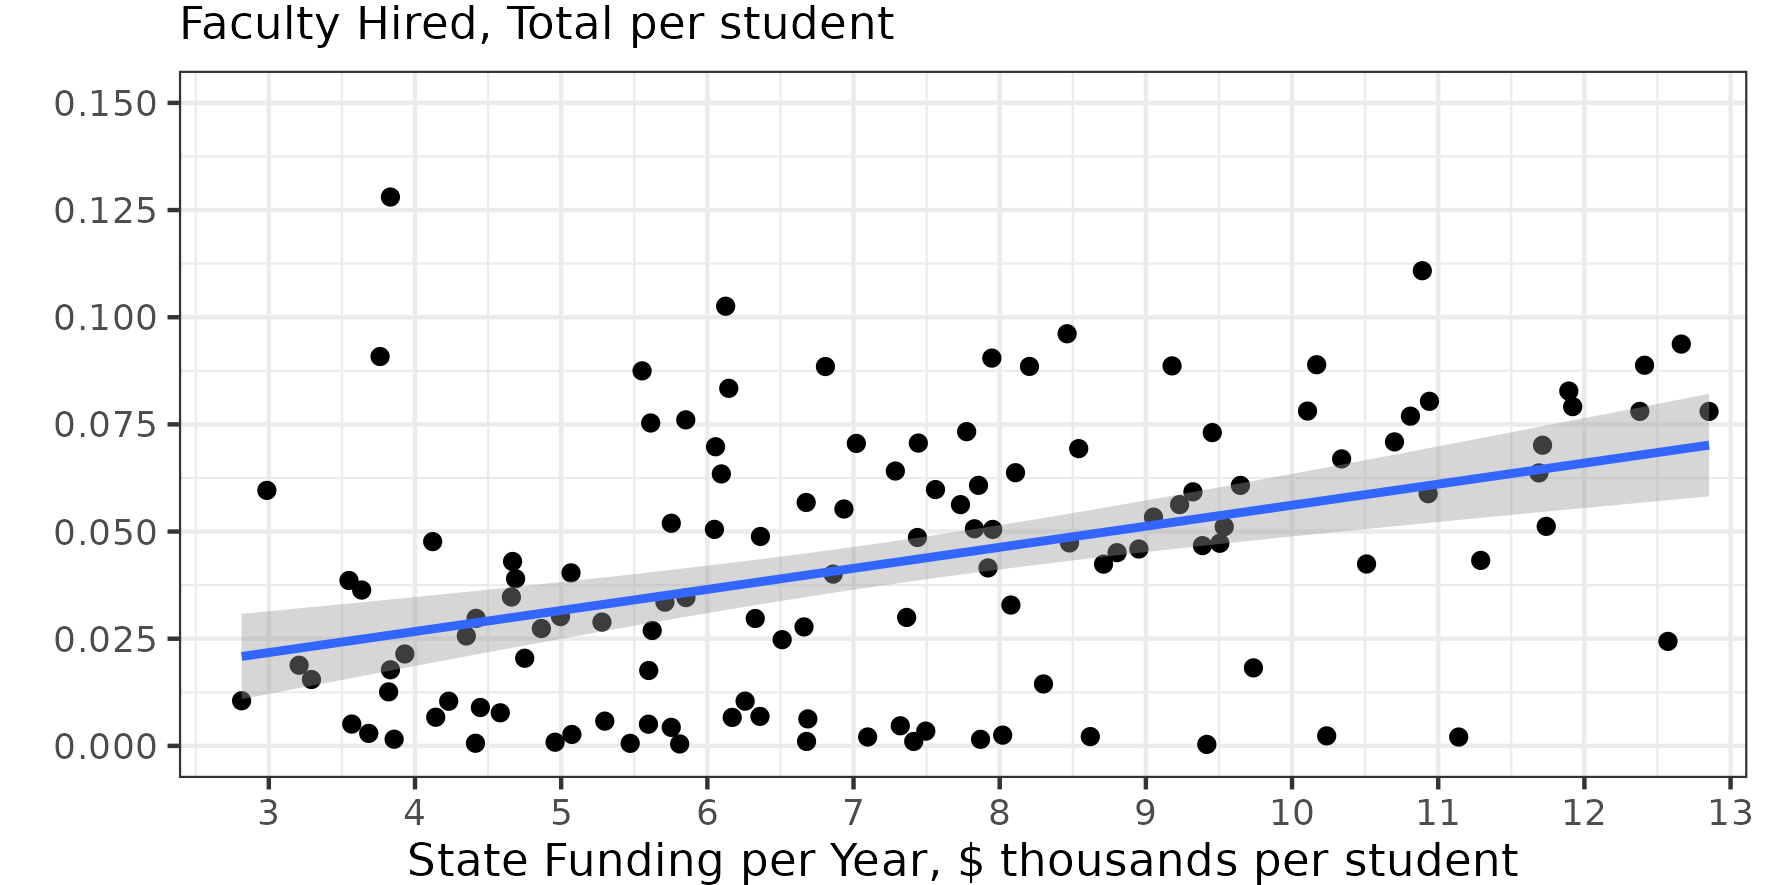
\includegraphics[width=0.75\textwidth]{figures/hiring-correlation.png}
    \label{fig:hiring-correlation}
    \justify
    \footnotesize
    \textbf{Note}:
    This figure shows the correlation between total state funding per student and total professors hired, 2010--2021.
    Funding data are taken from IPEDS, and data on professor hiring  from \cite{wapman2022quantifying,wapman2022zenodo}.
\end{figure}

\begin{table}[h!]
    \singlespacing
    \centering
    \caption{OLS and 2SLS Estimates for Professor Hiring, Total for 2011--2020.}
    \makebox[\textwidth][c]{
\begin{tabular}{@{\extracolsep{5pt}}lcccccc} 
\\[-1.8ex]\hline 
\hline \\[-1.8ex] 
 & \multicolumn{6}{c}{Dependent Variable: Professor Hiring Count} \\ 
\cline{2-7} 
\\[-1.8ex] & \multicolumn{2}{c}{Men} & \multicolumn{2}{c}{Women} & \multicolumn{2}{c}{Total} \\ 
 & OLS & 2SLS & OLS & 2SLS & OLS & 2SLS \\ 
\\[-1.8ex] & (1) & (2) & (3) & (4) & (5) & (6)\\ 
\hline \\[-1.8ex] 
 State Funding & 0.805 & 1.308 & 0.845 & 1.325 & 0.848 & 1.306 \\ 
  & (0.222) & (0.365) & (0.235) & (0.335) & (0.220) & (0.352) \\ 
 \hline \\[-1.8ex] 
Observations & 157 & 157 & 157 & 157 & 157 & 157 \\ 
R$^{2}$ & 0.396 & 0.366 & 0.415 & 0.383 & 0.408 & 0.381 \\ 
\hline 
\hline \\[-1.8ex] 
\end{tabular} 
}
    \label{tab:hiring-shock-reg}
    \justify
    \footnotesize
    \textbf{Note}: 
    This table show the second stage 2SLS estimates of regression specification \eqref{eqn:secondstage}, showing the effect of state funding changes on the number of faculty hires (per student) total for 2011--2021 at US public universities, using the funding shift-share to instrument for state funding.
    Yearly variation in total hires is not observed here, so only the total hires across 2011--2021 for 157 universities, can be considered.
    Each observation is a public university across the years 2011--2021, where data on total funding across 2011--2021 come from IPEDS and faculty count total from \citep{wapman2022quantifying,wapman2022zenodo}.
    The panels show the effect of a $1$\% change in state funding per student at the university (total for 2011--2021) on the number of new faculty hires by gender (and all).
    Standard errors are clustered at the state level, and state fixed effects are included through--out.
\end{table}

\newpage
\subsection{Robustness Checks}

\begin{table}[H]
    \singlespacing
    \centering
    \caption{Effects of State Funding on Faculty Counts, IPEDS 1990--2021, IV Estimates by Institution Selectivity.}

    \textbf{Panel A: units in \$ per student}

    \makebox[\textwidth][c]{
        \begin{tabular}{@{\extracolsep{5pt}}lcccccl} 
            \\[-1.8ex]\hline 
            \hline \\[-1.8ex]
            & First-stage & Lecturers & Asst. Professors & Full Professors & All Faculty & Observations \\ 
            \cline{2-7} 
            \\[-1.8ex]
            % latex table generated in R 4.3.1 by xtable 1.8-4 package
% Tue Apr 30 17:23:04 2024
  &  &  &  &  &  &  \\ 
  Most Selective: & -1.804 & 0.176 & 5.421 & 3.011 & 14.298 & 367 \\ 
   & (0.178) & (1.836) & (2.389) & (4.015) & (10.112) &  \\ 
   & [13036.59] & [0.004] & [0.011] & [0.033] & [0.05] &  \\ 
  Selective: & -5.555 & -0.089 & 0.025 & 0.044 & 0.022 & 815 \\ 
   & (0.324) & (0.019) & (0.006) & (0.004) & (0.003) &  \\ 
   & [12084.012] & [0.005] & [0.011] & [0.03] & [0.046] &  \\ 
  Unranked: & -7.264 & -0.058 & 0.018 & 0.017 & 0.008 & 15830 \\ 
   & (0.272) & (0.005) & (0.002) & (0.002) & (0.001) &  \\ 
   & [10206.27] & [0.006] & [0.012] & [0.022] & [0.041] &  \\ 
  
            \\[-1.8ex] \hline 
            \hline 
        \end{tabular}}
    
        \vspace{0.2cm}
    \textbf{Panel B: units in log \$ per student}
    
    \makebox[\textwidth][c]{
        \begin{tabular}{@{\extracolsep{5pt}}lcccccl} 
            \\[-1.8ex]\hline 
            \hline \\[-1.8ex]
            & First-stage & Lecturers & Asst. Professors & Full Professors & All Faculty & Observations \\ 
            \cline{2-7} 
            \\[-1.8ex]
            % latex table generated in R 4.3.1 by xtable 1.8-4 package
% Tue Apr 30 17:23:04 2024
  &  &  &  &  &  &  \\ 
  Most Selective: & -0.944 & -0.201 & 0.162 & 0.001 & -0.01 & 367 \\ 
   & (0.043) & (0.134) & (0.069) & (0.041) & (0.037) &  \\ 
   & [13036.59] & [0.004] & [0.011] & [0.033] & [0.05] &  \\ 
  Selective: & -1.067 & -0.465 & 0.129 & 0.229 & 0.116 & 815 \\ 
   & (0.022) & (0.092) & (0.031) & (0.018) & (0.016) &  \\ 
   & [12084.012] & [0.005] & [0.011] & [0.03] & [0.046] &  \\ 
  Unranked: & -0.965 & -0.436 & 0.137 & 0.131 & 0.062 & 15830 \\ 
   & (0.019) & (0.032) & (0.015) & (0.012) & (0.009) &  \\ 
   & [10206.27] & [0.006] & [0.012] & [0.022] & [0.041] &  \\ 
  
            \\[-1.8ex] \hline 
            \hline 
        \end{tabular}}
    \label{tab:facultycount-heterogeneity}
    \justify
    \footnotesize
    \textbf{Note}:
    These tables show the IV estimates of regression specification \eqref{eqn:secondstage}, 
    in the same manner as \autoref{tab:facultycount-shock-reg}, but restricting to institutions ranked as most selective, selective, and unranked by \cite{barrons2009} --- and including state
    The first column presents the coefficient between state funding and shift-share IV, which is a string first-stage among every level of selectivity for public universities.
    The other columns show the coefficient between state funding the count of faculty per students.
    For example, Row 1 of panel B shows that a $10\%$ cut in the state shift-share leads to a fall of $9.44\%$ in state funding for the public universities ranked as ``most selective.''
    Standard errors for the coefficient estimates are in brackets, and the outcome mean are in square brackets beneath.
\end{table}

\begin{table}[H]
    \singlespacing
    \centering
    \caption{First-stage Robustness Checks for Effects of State Funding Shift-Share on State Funding, OLS Estimates.}
    \makebox[\textwidth][c]{
\begin{tabular}{@{\extracolsep{5pt}}lcc} 
\\[-1.8ex]\hline 
\hline \\[-1.8ex] 
 & \multicolumn{2}{c}{Dependent Variable: State Funding} \\ 
\cline{2-3} 
 & Raw Count Units & Log Units \\ 
\\[-1.8ex] & (1) & (2)\\ 
\hline \\[-1.8ex] 
 State Funding & $-$1.299 & $-$1.050 \\ 
  & (0.172) & (0.041) \\ 
  State Funding, Base Share \% & $-$95.489 & $-$0.895 \\ 
  & (40.941) & (0.141) \\ 
  Acceptance Rate, \% & $-$13.540 & $-$0.012 \\ 
  & (15.208) & (0.046) \\ 
  6--Year Completion Rate, \% & 69.341 & 0.148 \\ 
  & (23.718) & (0.074) \\ 
  Tuition Revenue, \$ millions & 1.223 & 0.350 \\ 
  & (1.433) & (0.040) \\ 
  Enrolment, FTE thousands & $-$4.748 & $-$0.669 \\ 
  & (58.129) & (0.055) \\ 
  State Enrolment, thousands & 2.215 & 0.258 \\ 
  & (1.236) & (0.053) \\ 
  Percent of State Enrolment & 0.803 & 0.0003 \\ 
  & (3.356) & (0.0001) \\ 
 \hline \\[-1.8ex] 
Units  & Raw counts & Log, \% terms \\ 
F stat. & 57.356 & 660.878 \\ 
State + Year fixed effects? & Yes & Yes \\ 
Observations & 13,687 & 13,687 \\ 
R$^{2}$ & 0.382 & 0.453 \\ 
\hline 
\hline \\[-1.8ex] 
\end{tabular} 
}
    \label{tab:firststage-robustness-checks}
    \justify
    \footnotesize
    \textbf{Note}:
    These tables show the second stage OLS and 2SLS estimates of regression specification \eqref{eqn:firststage}, showing the effect of state funding shift-share on each university's state funding.
    This table differs from the main analysis by replacing University $+$ Year fixed effects with State $+$ Year fixed effects, measuring enrolment in full-time equivalent (FTE), and including controls for (1)
    State Funding as a percent of total funding in base period, (2) acceptance rate in mid-2000s, (3) 6--year completion rate in mid-2000s, (4) tuition revenue, (5) enrolment measured by full-time equivalent FTE, (6) total public university enrolment in the entire state, (7) percent of public university enrolment for the state enrolled at this university.
    The first column uses the raw count specification, and the second column uses the $\log$ specification for percentage terms.
\end{table}

\begin{table}[H]
    \singlespacing
    \centering
    \caption{Robustness Checks for Effects of State Funding Cuts on Faculty Composition, OLS and 2SLS Estimates in $\log$ Units.}
    \makebox[\textwidth][c]{
        %\small
        
\begin{tabular}{@{\extracolsep{5pt}}lcccccccc} 
\\[-1.8ex]\hline 
\hline \\[-1.8ex] 
 & \multicolumn{8}{c}{Dependent Variable: Log Faculty Count per Students, by Position} \\ 
\cline{2-9} 
\\[-1.8ex] & \multicolumn{2}{c}{Lecturers} & \multicolumn{2}{c}{Asst. Professors} & \multicolumn{2}{c}{Full Professors} & \multicolumn{2}{c}{All Faculty} \\ 
 & OLS & 2SLS & OLS & 2SLS & OLS & 2SLS & OLS & 2SLS \\ 
\\[-1.8ex] & (1) & (2) & (3) & (4) & (5) & (6) & (7) & (8)\\ 
\hline \\[-1.8ex] 
 State Funding & $-$0.116 & $-$0.352 & 0.072 & 0.069 & 0.147 & 0.104 & 0.095 & 0.038 \\ 
  & (0.042) & (0.088) & (0.026) & (0.048) & (0.050) & (0.022) & (0.038) & (0.023) \\ 
  State Funding, Base Share \% & $-$0.053 & $-$0.042 & $-$0.022 & $-$0.022 & 0.075 & 0.077 & 0.025 & 0.028 \\ 
  & (0.160) & (0.172) & (0.049) & (0.049) & (0.047) & (0.047) & (0.037) & (0.038) \\ 
  Acceptance Rate, \% & 0.015 & 0.00004 & 0.004 & 0.004 & $-$0.012 & $-$0.015 & $-$0.013 & $-$0.016 \\ 
  & (0.077) & (0.082) & (0.043) & (0.044) & (0.038) & (0.039) & (0.029) & (0.031) \\ 
  6--Year Completion Rate, \% & $-$0.029 & 0.023 & 0.130 & 0.130 & 0.241 & 0.250 & 0.156 & 0.169 \\ 
  & (0.112) & (0.125) & (0.034) & (0.033) & (0.036) & (0.034) & (0.021) & (0.024) \\ 
  Tuition Revenue, \$ millions & 0.347 & 0.421 & 0.046 & 0.046 & 0.235 & 0.248 & 0.215 & 0.233 \\ 
  & (0.153) & (0.163) & (0.053) & (0.055) & (0.033) & (0.033) & (0.038) & (0.033) \\ 
  Enrolment, FTE thousands & $-$0.580 & $-$0.698 & $-$0.223 & $-$0.224 & $-$0.278 & $-$0.300 & $-$0.336 & $-$0.364 \\ 
  & (0.179) & (0.198) & (0.062) & (0.065) & (0.039) & (0.036) & (0.048) & (0.037) \\ 
  State Enrolment, thousands & 0.232 & 0.331 & $-$0.112 & $-$0.111 & $-$0.196 & $-$0.178 & $-$0.102 & $-$0.079 \\ 
  & (0.189) & (0.177) & (0.068) & (0.069) & (0.061) & (0.050) & (0.046) & (0.032) \\ 
  Percent of State Enrolment & 0.150 & 0.417 & 0.021 & 0.024 & $-$0.021 & 0.027 & 0.095 & 0.159 \\ 
  & (0.591) & (0.595) & (0.177) & (0.183) & (0.168) & (0.130) & (0.158) & (0.135) \\ 
 \hline \\[-1.8ex] 
Outcome Mean & 0.681 & 0.681 & 1.394 & 1.394 & 2.666 & 2.666 & 4.816 & 4.816 \\ 
Observations & 13,687 & 13,687 & 13,687 & 13,687 & 13,687 & 13,687 & 13,687 & 13,687 \\ 
R$^{2}$ & 0.341 & 0.327 & 0.440 & 0.440 & 0.438 & 0.433 & 0.543 & 0.529 \\ 
\hline 
\hline \\[-1.8ex] 
\end{tabular} 
}
    \label{tab:facultycount-robustness-checks}
    \justify
    \footnotesize
    \textbf{Note}:
    These tables show the second stage OLS and 2SLS estimates of regression specification \eqref{eqn:secondstage}, showing the effect of state funding changes on number of faculty per student in Illinois universities, using the funding shift-share to instrument for state funding in the columns labelled 2SLS.
    This table differs from the main analysis by replacing University $+$ Year fixed effects with State $+$ Year fixed effects, measuring enrolment in full-time equivalent (FTE), and including controls for (1)
    State Funding as a percent of total funding in base period, (2) acceptance rate in mid-2000s, (3) 6--year completion rate in mid-2000s, (4) tuition revenue, (5) enrolment measured by full-time equivalent FTE, (6) total public university enrolment in the entire state, (7) percent of public university enrolment for the state enrolled at this university.
\end{table}


\begin{table}[H]
    \singlespacing
    \centering
    \caption{Robustness Checks for Effects of State Funding Cuts on Faculty Composition, OLS and 2SLS Estimates in Raw Count Units.}
    \makebox[\textwidth][c]{
        \small
        
\begin{tabular}{@{\extracolsep{5pt}}lcccccccc} 
\\[-1.8ex]\hline 
\hline \\[-1.8ex] 
 & \multicolumn{8}{c}{Dependent Variable: Faculty Count per 1,000 Students, by Position} \\ 
\cline{2-9} 
\\[-1.8ex] & \multicolumn{2}{c}{Lecturers} & \multicolumn{2}{c}{Asst. Professors} & \multicolumn{2}{c}{Full Professors} & \multicolumn{2}{c}{All Faculty} \\ 
 & OLS & 2SLS & OLS & 2SLS & OLS & 2SLS & OLS & 2SLS \\ 
\\[-1.8ex] & (1) & (2) & (3) & (4) & (5) & (6) & (7) & (8)\\ 
\hline \\[-1.8ex] 
 State Funding & $-$1.001 & $-$1.641 & 1.032 & 4.573 & 7.128 & 6.836 & 7.213 & 10.746 \\ 
  & (0.461) & (1.345) & (0.397) & (2.094) & (1.212) & (3.097) & (1.396) & (5.276) \\ 
  State Funding, Base Share \% & 55.056 & 57.126 & 15.654 & 4.200 & $-$38.543 & $-$37.598 & 18.057 & 6.627 \\ 
  & (24.373) & (25.604) & (35.625) & (37.658) & (53.606) & (51.900) & (95.185) & (95.017) \\ 
  Acceptance Rate, \% & $-$7.862 & $-$8.694 & 6.849 & 11.450 & $-$41.508 & $-$41.888 & $-$53.375 & $-$48.783 \\ 
  & (10.581) & (9.949) & (9.243) & (14.230) & (21.648) & (20.581) & (26.159) & (29.083) \\ 
  6--Year Completion Rate, \% & 8.357 & 12.754 & 21.899 & $-$2.429 & 169.846 & 171.853 & 202.607 & 178.329 \\ 
  & (18.767) & (21.069) & (13.444) & (23.497) & (42.483) & (45.635) & (39.685) & (47.031) \\ 
  Tuition Revenue, \$ millions & 0.185 & 0.186 & 0.123 & 0.118 & 0.215 & 0.216 & 0.622 & 0.617 \\ 
  & (0.035) & (0.035) & (0.027) & (0.028) & (0.064) & (0.064) & (0.137) & (0.137) \\ 
  Enrolment, FTE thousands & 2.580 & 2.575 & 7.029 & 7.060 & 22.975 & 22.972 & 32.420 & 32.450 \\ 
  & (0.858) & (0.848) & (0.595) & (0.554) & (1.272) & (1.276) & (1.925) & (1.900) \\ 
  State Enrolment, thousands & 0.088 & 0.086 & $-$0.061 & $-$0.054 & $-$0.218 & $-$0.218 & $-$0.188 & $-$0.182 \\ 
  & (0.021) & (0.021) & (0.020) & (0.020) & (0.069) & (0.067) & (0.098) & (0.098) \\ 
  Percent of State Enrolment & $-$7.625 & $-$6.651 & 126.755 & 121.370 & 168.080 & 168.525 & 255.309 & 249.936 \\ 
  & (48.023) & (48.705) & (42.249) & (37.381) & (72.631) & (72.682) & (105.737) & (102.570) \\ 
 \hline \\[-1.8ex] 
Outcome Mean & 59.253 & 59.253 & 116.121 & 116.121 & 269.103 & 269.103 & 452.507 & 452.507 \\ 
Observations & 13,687 & 13,687 & 13,687 & 13,687 & 13,687 & 13,687 & 13,687 & 13,687 \\ 
R$^{2}$ & 0.647 & 0.646 & 0.861 & 0.845 & 0.942 & 0.942 & 0.954 & 0.954 \\ 
\hline 
\hline \\[-1.8ex] 
\end{tabular} 
}
    \label{tab:facultycount-rawcount-robustness-checks}
    \justify
    \footnotesize
    \textbf{Note}:
    These tables show the second stage OLS and 2SLS estimates of regression specification \eqref{eqn:secondstage}, showing the effect of state funding changes on count of faculty in Illinois universities, using the funding shift-share to instrument for state funding in the columns labelled 2SLS.
    This table differs from the main analysis by replacing University $+$ Year fixed effects with State $+$ Year fixed effects, measuring enrolment in full-time equivalent (FTE), and including controls for (1)
    State Funding as a percent of total funding in base period, (2) acceptance rate in mid-2000s, (3) 6--year completion rate in mid-2000s, (4) tuition revenue, (5) enrolment measured by full-time equivalent FTE, (6) total public university enrolment in the entire state, (7) percent of public university enrolment for the state enrolled at this university.
\end{table}

\begin{table}[H]
    \singlespacing
    \centering
    \caption{Effects of State--Wide Funding Changes on Private University Faculty Counts, IPEDS 1990--2021, OLS and 2SLS Estimates.}

    \textbf{Panel A: units in \$ per student}

    \makebox[\textwidth][c]{
\begin{tabular}{@{\extracolsep{5pt}}lcccccccc} 
\\[-1.8ex]\hline 
\hline \\[-1.8ex] 
 & \multicolumn{8}{c}{Dependent Variable: Faculty Count per 1,000 Students, by Position} \\ 
\cline{2-9} 
\\[-1.8ex] & \multicolumn{2}{c}{Lecturers} & \multicolumn{2}{c}{Asst. Professors} & \multicolumn{2}{c}{Full Professors} & \multicolumn{2}{c}{All Faculty} \\ 
 & OLS & 2SLS & OLS & 2SLS & OLS & 2SLS & OLS & 2SLS \\ 
\\[-1.8ex] & (1) & (2) & (3) & (4) & (5) & (6) & (7) & (8)\\ 
\hline \\[-1.8ex] 
 State Funding & 0.002 & $-$0.099 & 0.003 & 0.037 & 0.005 & $-$0.060 & 0.011 & $-$0.099 \\ 
  & (0.002) & (0.193) & (0.001) & (0.190) & (0.003) & (0.176) & (0.006) & (0.406) \\ 
 \hline \\[-1.8ex] 
Outcome Mean & 12.392 & 12.392 & 35.058 & 35.058 & 62.593 & 62.593 & 111.495 & 111.495 \\ 
Observations & 25,309 & 25,309 & 25,309 & 25,309 & 25,309 & 25,309 & 25,309 & 25,309 \\ 
R$^{2}$ & 0.617 & 0.415 & 0.788 & 0.778 & 0.944 & 0.937 & 0.904 & 0.897 \\ 
\hline 
\hline \\[-1.8ex] 
\end{tabular} 
}
    
    \textbf{Panel B: units in log \$ per student}
    
    \makebox[\textwidth][c]{
\begin{tabular}{@{\extracolsep{5pt}}lcccccccc} 
\\[-1.8ex]\hline 
\hline \\[-1.8ex] 
 & \multicolumn{8}{c}{Dependent Variable: Log Faculty Count per Students, by Position} \\ 
\cline{2-9} 
\\[-1.8ex] & \multicolumn{2}{c}{Lecturers} & \multicolumn{2}{c}{Asst. Professors} & \multicolumn{2}{c}{Full Professors} & \multicolumn{2}{c}{All Faculty} \\ 
 & OLS & 2SLS & OLS & 2SLS & OLS & 2SLS & OLS & 2SLS \\ 
\\[-1.8ex] & (1) & (2) & (3) & (4) & (5) & (6) & (7) & (8)\\ 
\hline \\[-1.8ex] 
 State Funding & 0.412 & $-$0.728 & 0.366 & $-$1.716 & 0.394 & $-$0.331 & 0.381 & $-$1.563 \\ 
  & (0.079) & (6.354) & (0.058) & (4.346) & (0.063) & (1.819) & (0.060) & (3.969) \\ 
 \hline \\[-1.8ex] 
Outcome Mean & 0.744 & 0.744 & 1.935 & 1.935 & 3.075 & 3.075 & 5.824 & 5.824 \\ 
Observations & 25,309 & 25,309 & 25,309 & 25,309 & 25,309 & 25,309 & 25,309 & 25,309 \\ 
R$^{2}$ & 0.639 & 0.549 & 0.741 & 0.002 & 0.819 & 0.734 & 0.845 & $-$0.125 \\ 
\hline 
\hline \\[-1.8ex] 
\end{tabular} 
}

    \label{tab:facultycount-shock-private-robustness}
    \justify
    \footnotesize
    \textbf{Note}:
    These tables show the second stage OLS and 2SLS estimates of regression specification \eqref{eqn:secondstage}, among private universities --- as described in \autoref{sec:results-robustness}.
    Each observation is a public university-year, in the IPEDS data.
    Panel A shows the effect of a fall in state funding \$$-1,000$ per student on the number of professors --- i.e.,
    an extra \$$1,000$ per student leads to 6 fewer lecturers according to column 2.
    Panel B shows the effect of a $10$\% change in state funding per student at the university on the 10\% change in the number of professors per students --- i.e.,
    an extra 10\% of state funding per student leads to 4.37\% fewer lecturers per student according to column 2.
    Outcome-mean is the mean of the outcome, for Panel A the number of professors per student, for Panel B the number of faculty per student.
    Panel B uses $\log$ faculty count per student as the outcome, though the outcome mean is count of faculty per student (not in $\log$ terms).
    Standard errors are clustered at the state-year level, and university $+$ year fixed effects are included through--out.
\end{table}

%\newpage
%\subsection{Rates of Substitution}
%\label{sec:appendix-substitution}
%The funding elasticities can be used to recover the marginal rate of substitution between two outcomes.
%For example, write $Y^1$ for the number of lecturers per student at a university, and $Y^2$ for the number of full professors.
%I use the above approaches to estimate the funding elasticities, where $\% \Delta$ denotes percent change.
%\[ \beta_1 = \frac{\% \Delta Y^1}{\% \Delta X}
%\text{, and }
%\beta_2 = \frac{\% \Delta Y^2}{\% \Delta X} \]
%As such, it is possible to recover the elasticity for substitution between lecturers and full professors by the universities via the respective funding elasticities.
%\[ \frac{\% \Delta Y^1}{\% \Delta Y^2}
%= \frac{\% \Delta Y^1 / \% \Delta X}{\% \Delta Y^2 / \% \Delta X}
%= \frac{\beta_1}{\beta_2} \]
%I present results for the rates of substitution between different levels of faculty by this approach, dividing the relevant coefficient estimates and presenting standard errors calculated by a non-parametric bootstrap.
%In practice, this corresponds to division of the estimates of the elasticity for employment of professors (by rank) with respect to state funding, presented in Panel B \autoref{tab:facultycount-shock-reg}, and bootstrapping the results to generate standard errors and confidence intervals.
%% https://stackoverflow.com/questions/63777368/computing-the-standard-error-when-dividing-coefficients-of-different-regressions
%
%The implied marginal rate of substitution between lecturers and assistant professors is estimated as -3.26 (standard error 0.50), based on 10,000 bootstrap samples.
%This means that public universities increased their number lecturers per student by 3.26\% when they decreased their count of assistant professors, on average and subject to the changes in state funding they experienced 1990--2017.
%Between lecturers and full professors the rate of substitution is -3.19 (0.34), which implies that universities substitute between lecturers and full professors in the same way.
%Between assistant and full professors the rate of substitution is 0.99 (0.11), which intuitively implies that universities treated assistant and full professors (i.e., those before and after tenure in the tenure system) as complements.
%
%"Calculated point est for substitution between lecturers + ast profs" 
%                                                                      
%                                                  "-3.26372574229461" 
%                                                                      
%                                                           "with SEs" 
%                                                                      
%                                                  "0.501721750806993" 
%                                                                      
%                                                        "and 95 % CI" 
%                                                                 2.5% 
%                                                  "-4.38380704259523" 
%                                                                97.5% 
%                                                  "-2.40372605889863"

                                                                      
% "Calculated point est for substitution between lecturers + full profs" 
%                                                                       
%                                                    "-3.1876596143219" 
%                                                                       
%                                                            "with SEs" 
%                                                                       
%                                                   "0.340087353132307" 
%                                                                       
%                                                         "and 95 % CI" 
%                                                                  2.5% 
%                                                   "-3.88637781601822" 
%                                                                 97.5% 
%                                                   "-2.56722681973736" 

% "Calculated point est for substitution between ast + full profs" 
%                                                                  
%                                              "0.990674987591129" 
%                                                                  
%                                                       "with SEs" 
%                                                                  
%                                              "0.116874891784044" 
%                                                                  
%                                                    "and 95 % CI" 
%                                                             2.5% 
%                                              "0.771569155168642" 
%                                                            97.5% 
%                                               "1.23151772759759" 
